\section{Circular Arc Geometry}
\label{sect:circular-arc-geometry}

A 3-tuple ${(P, Q, \varphi)}$ uniquely determines a circular arc ${\Gamma(P, Q, \varphi)}$. Here ${P, Q \in \mathbb{R}^2}$ are its distinct endpoints, and ${\varphi \in (-180\degrees, 180\degrees)}$ is the (signed) angle from the chord ${PQ}$ to the arc's tangent in ${P}$.

Drawing a circular arc with ${\varphi > 0 \degrees}$ starting in ${P}$ requires a clockwise motion; hence those arcs shall be called \emph{clockwise}. Similarly, arcs shall be called \emph{counterclockwise} for ${\varphi < 0 \degrees}$. For ${\varphi = 0 \degrees}$ the arc degenerates into the straight line segment connecting ${P}$ and ${Q}$. \Cref{fig:circular-arc-geometry} outlines important properties of a circular arc.
%
\begin{figure}[H]
  \centering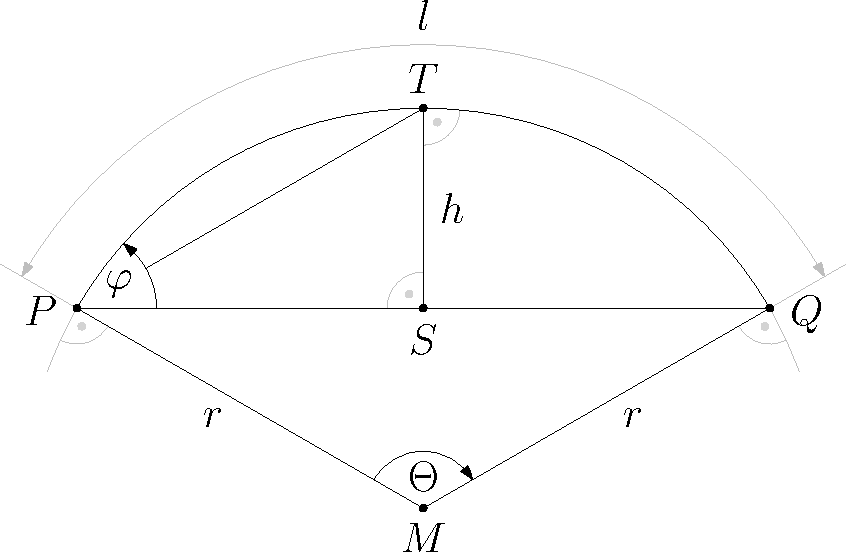
\includegraphics[width=0.6\textwidth]{Resources/Figures/Clockwise-Circular-Arc.pdf}
  \caption{Geometry of a clockwise circular arc.}
  \label{fig:circular-arc-geometry}
\end{figure}



\noindent
The \emph{central angle} ${\Theta}$ is the (signed) angle which the arc subtends at the center of the circle. For clockwise arcs the central angle is negative; for counterclockwise arcs it is positive:
%
\begin{equation*}
  \Theta = -2 \varphi
\end{equation*}



\noindent
The \emph{arc height} ${h}$ is the (signed) perpendicular distance from the arc's midpoint ${T}$ to the chord ${PQ}$ connecting its endpoints. For clockwise arcs the arc height is positive; for counterclockwise arcs it is negative. When cutting ${\Gamma}$ in half, the circular arc ${\Gamma'}$ with chord ${PT}$ has ${\Theta' = \frac{\Theta}{2}}$ and ${\varphi' = \frac{\varphi}{2}}$. Therefore we find ${\angle SPT = \varphi - \frac{\varphi}{2}}$, and we can write the arc height as
%
\begin{equation*}
  h \: = \: \segment{PS} \cdot \eval{\tan}{\angle SPT} \; = \; \frac{1}{2} \segment{PQ} \cdot \eval{\tan}{\frac{\varphi}{2}}.
\end{equation*}



\noindent
The \emph{arc radius} ${r}$ and \emph{arc center} ${M}$ are, respectively, the radius and center of the circle which the arc is a slice of. We find them to be
%
\begin{align*}
  r(\varphi \neq 0 \degrees) &= \abs{\frac{\segment{PS}}{\eval{\sin}{\varphi}}} = \abs{\frac{\segment{PQ}}{2 \eval{\sin}{\varphi}}}
  \intertext{and}
  M(\varphi \neq 0 \degrees) &= P + R(\varphi - 90 \degrees)
    \cdot \frac{\longvec{PQ}}{2 \eval{\sin}{\varphi}},
\end{align*}
%
where ${R(\psi)}$ is the matrix rotating a column vector by ${\psi}$ in the counterclockwise direction. Note that for ${\varphi = 0 \degrees}$, both radius ${r}$ and center ${M}$ are undefined.



The \emph{arc length} ${l}$ is the distance between the arc's endpoints ${P}$ and ${Q}$ along the arc. It is a portion of the respective circle's circumference:
%
\begin{equation*}
  l(\varphi \neq 0 \degrees) = \abs{\frac{\Theta}{360 \degrees} \cdot 2 \pi r} = \abs{\frac{\varphi}{180 \degrees} \cdot \frac{\pi \cdot \segment{PQ}}{\eval{\sin}{\varphi}}}
\end{equation*}



\noindent
For ${\varphi = 0 \degrees}$, above equation for arc length ${l}$ is undefined. We shall continuously extend it to ${\varphi = 0 \degrees}$ using the limit ${\lim_{\varphi \to 0 \degrees}}$:
%
\begin{equation*}
  l(\varphi = 0 \degrees) \coloneqq \lim_{\varphi \to 0 \degrees} l(\varphi) = \segment{PQ}
\end{equation*}
%
This extension also matches our intuition of the arc degenerating into a straight line segment for ${\varphi \to 0 \degrees}$.
